
%(BEGIN_QUESTION)
% Copyright 2008, Tony R. Kuphaldt, released under the Creative Commons Attribution License (v 1.0)
% This means you may do almost anything with this work of mine, so long as you give me proper credit

A water-cooled generator at a power plant has two sources of cooling water flow, each source equipped with a flow switch that returns to its normally-open status if the water flow through the pipe stops.  If either water source ceases supplying cooling water to the generator (for whatever reason), that flow switch will de-actuate and turn the warning light on.  This is all that is required, as the generator will still receive adequate cooling from only one source.  If both water sources cease supplying water, however, a ``trip'' solenoid will energize to shut down the generator before it overheats:

$$\includegraphics[width=15.5cm]{i03199x01.eps}$$

One day the warning light comes on, but there is still cooling water flowing to the generator so it does not shut down.  You are asked to determine what the problem is, while maintaining the system in an operating condition (i.e. you are not allowed to shut off control power or do anything else that might shut down the generator). 

\vskip 10pt

First, assess whether or not the following diagnostic test would provide any useful information about the fault: {\it suppose a technician connects an AC voltmeter between terminals TP6 and L2}.  Will this test provide information to help us diagnose the nature and/or location of the fault?  Why or why not?

\vskip 30pt

Next, propose a diagnostic test that would definitely provide useful information about either the location or the nature of the fault in this system.  Your proposal must identify the meaning of at least one possible result of the test (e.g. {\it ``If I jumper terminals $X$ and $Y$ together and I measure a decrease in source voltage, it means the fault must be a short somewhere in branch A-B-C of the circuit''}).  Remember that the best diagnostic test is one that yields definitive answers no matter what its result might be.  Directly checking a suspected component is {\it not} a good diagnostic test, unless there are simply no other options!




\vfil 

\underbar{file i03199}
\eject
%(END_QUESTION)





%(BEGIN_ANSWER)

This is a graded question -- no answers or hints given!

%(END_ANSWER)





%(BEGIN_NOTES)

The 120 volt AC measurement across the warning light's terminals is not a useful test, because we already known it's getting power due to the fact that it is currently lit.

\vskip 10pt

\noindent
More useful diagnostic tests include the following:

\item{} Measure voltage between TP2 and L2 (if no voltage, either flow A is too low or there is an ``open'' fault between L1 and TP2
\item{} Measure voltage between TP4 and L2 (if no voltage, either flow B is too low or there is an ``open'' fault between L1 and TP4
\end{itemize}


%INDEX% Troubleshooting review: electric circuits

%(END_NOTES)


